\begin{abstract}
\noindent Adaptive artificial-intelligence systems are described in vague terms
--- \emph{self-improving}, \emph{resilient}, \emph{agentic} --- that
obscure the structural constraints under which such systems can actually
be viable. This paper identifies eight principles that bound the design
space of adaptive AI architectures. Six are established physical and
informational laws --- the Second Law of Thermodynamics, Ashby's Law of
Requisite Variety, Shannon's information theory, the Principle of Least
Action, Lyapunov stability, and the power-law distribution of system
events. Two are original frameworks proposed by the author for the
operator-cognitive performance layer of high-consequence systems:
\emph{Individual-Baseline Variance Modeling} and \emph{Precision
Perturbation Without Variance Compression}. The eight principles operate
as architectural design constraints, not as a theory of intelligence.
The first six are illustrated with their operational form inside MILO, a
patent-pending adaptive AI orchestrator developed by the author and
submitted to the U.S. Department of Energy under the Genesis Mission;
the seventh and eighth are v.5 design-stage frameworks, not shipped
operator-monitoring features. The synthesis is consistent with, and
complementary to, Friston's Free Energy Principle, Beer's Viable System
Model, and recent thermodynamics-adjacent AI work; it differs in that
the eight principles are used as design-time constraints on
architectural choices, not as a unified explanation of intelligence.
\end{abstract}

\noindent\textbf{Keywords:} adaptive AI, architectural constraints, cybernetics,
Lyapunov-style bounded response, antifragility, human-in-the-loop,
industrial AI orchestration\par

\textbf{Highlights.}

\begin{itemize}
\tightlist
\item
  Identifies eight structural principles that bound the design space of
  viable adaptive AI architectures, drawn from established physical,
  informational, control-theoretic, and statistical lineages.
\item
  Six principles apply established external laws (Second Law of
  Thermodynamics, Ashby's Law of Requisite Variety, Shannon Information
  Theory, Principle of Least Action, Lyapunov-style bounded response,
  Power-Law distribution).
\item
  Two original frameworks proposed by the author for the
  operator-cognitive performance layer: \emph{Individual-Baseline
  Variance Modeling} and \emph{Precision Perturbation Without Variance
  Compression} --- flagged as design-stage, pending empirical
  validation.
\item
  Synthesis is positioned as complementary to Friston's Free Energy
  Principle and Beer's Viable System Model but distinct --- design-time
  constraints on architectural choices, not a unified theory of
  intelligence.
\end{itemize}

\textbf{Index Terms:} adaptive AI architecture, structural principles,
cybernetics, control theory, Lyapunov stability, Ashby's Law of
Requisite Variety, Shannon Information Theory, antifragility, Power-Law
distribution, operator-cognitive modeling, viable system model.

\textbf{Plain Language Summary.} Adaptive AI systems are often described
in vague terms --- \emph{self-improving}, \emph{resilient},
\emph{agentic} --- that obscure what makes some such systems viable and
others fragile. This paper identifies eight engineering principles that
constrain the design space of viable adaptive AI architectures. Six are
established physical and informational laws (thermodynamic entropy,
Ashby's variety law, Shannon information theory, the principle of least
action, Lyapunov-style bounded response, and the power-law distribution
of system events) applied here as architectural design constraints
rather than as theories of intelligence. Two are original frameworks
proposed by the author for the operator-cognitive performance layer of
high-consequence systems: \emph{Individual-Baseline Variance Modeling}
and \emph{Precision Perturbation Without Variance Compression}. The
eight principles, taken together, separate adaptive AI orchestrators
that survive operational stress from those that fail it.

\textbf{Relevance to U.S. National Interest.} The principles articulated
here apply directly to the AI-enabled critical-infrastructure
environments identified by the DOE Genesis Mission --- advanced
manufacturing, grid reliability, autonomous systems, nuclear-facility
operations, and human-in-the-loop AI for high-consequence decision
support. Adaptive AI deployed in those environments without these
architectural constraints carries failure modes that the constraints
were established to prevent.

\textbf{Status of claims.} Six of the eight principles in this paper
apply established physical and informational laws as architectural
design constraints: the Second Law of Thermodynamics, Ashby's Law of
Requisite Variety \cite{ref6}, Shannon Information Theory \cite{ref7}, the
Principle of Least Action, Lyapunov stability \cite{ref8}, and the Power-Law
distribution of complex-system events \cite{ref9}. The mapping of each
principle to a specific orchestrator-level architectural choice is the
author's contribution and is subject to further validation; the laws
themselves are external references. Principles 7 and 8 ---
\emph{Individual-Baseline Variance Modeling} and \emph{Precision
Perturbation Without Variance Compression} --- are original frameworks
proposed by the author for the operator-cognitive performance layer of
high-consequence systems and are flagged in the paper as design-stage
frameworks pending empirical validation in shipped deployments. The
synthesis is consistent with prior work by Friston \cite{ref3}, Beer
\cite{ref4}, and the thermodynamic-AI literature \cite{ref5}; differences are
explicit in §2 and §5. This manuscript is a preprint prior to peer
review.

\textbf{About MILO.} MILO (Modular Intelligent Learning Orchestrator) is
a patent-pending adaptive AI orchestration architecture for
high-consequence critical-infrastructure environments. The full
architectural reference --- eight structural principles, eight
operational integrity constraints, the unifying viability principle, and
the trademark/patent status --- is maintained as a single canonical
document at https://github.com/jmontano1/milo-architecture (concept DOI:
10.5281/zenodo.20117025). Author contact: jmontano@jmautomated.com.

\begin{center}\rule{0.5\linewidth}{0.5pt}\end{center}

\subsection{1. Introduction}\label{introduction}

Adaptive AI architecture is most often described in language drawn from
the system's marketing rather than its physics. A system is
\emph{self-improving} because its developers say so; it is
\emph{resilient} because it has not yet failed visibly; it is
\emph{agentic} because it issues commands. These descriptors are claims
about capability, not about structural form. They do not tell an
engineer whether the system can survive a perturbation it was not
trained for, whether its internal variety matches the variety of the
environment it governs, whether its informational paths admit auditable
decisions, or whether its adaptation has any bounded stop condition.

The history of engineering offers a better discipline. Physical and
informational systems are not viable because they are aspirationally
well-intentioned; they are viable because their architecture obeys
constraints that have been established for decades --- in
thermodynamics, in classical mechanics, in cybernetics, in control
theory, in information theory, and in the empirical statistics of
complex systems. An adaptive AI architecture that ignores those
constraints inherits failure modes the constraints were discovered to
prevent.

This paper identifies eight such principles and argues that they
constitute structural constraints on the design space of viable adaptive
AI systems. Six are established laws applied as architectural design
constraints. Two are original frameworks proposed by the author for the
operator cognitive performance layer of high-consequence industrial
systems, where human decision context, cognitive load, fatigue, and
task-state misalignment can become material sources of operational
variance.

The eight principles are illustrated using MILO (Modular Intelligent
Learning Orchestrator), a patent-pending adaptive AI orchestration
system \cite{ref1} that the author has developed and submitted to the U.S.
Department of Energy under the Genesis Mission \cite{ref2}. MILO is the
working substrate for the first six principles and the design substrate
for the proposed v.5 operator-layer extension; the paper's contribution
is the principles, not the implementation. Where MILO is referenced, it
is referenced at the architectural level only.

The paper does not propose a new theory of intelligence. Several
frameworks --- Friston's Free Energy Principle and Active Inference
\cite{ref3}, Beer's Viable System Model \cite{ref4}, and thermodynamics-adjacent
AI explanation work \cite{ref5} --- already address broader explanatory or
diagnostic layers. The contribution here is narrower and more practical:
a set of design-time architectural constraints that, taken together,
separate viable adaptive AI orchestrations from systems that merely
claim viability.

\subsection{2. Background and Related
Work}\label{background-and-related-work}

The eight principles draw from five established intellectual lineages.
The Second Law of Thermodynamics, formalized by Clausius and refined by
Boltzmann, established entropy as the directional quantity governing
closed-system evolution. Ashby's Law of Requisite Variety \cite{ref6},
introduced in 1956 cybernetics, established that a regulator must
possess variety at least equal to the system it regulates. Shannon's
information theory \cite{ref7}, introduced in 1948, established the
channel-capacity bounds on noise-tolerant communication. The Principle
of Least Action, developed by Maupertuis, Lagrange, and Hamilton,
established that physical systems traverse trajectories of minimum
action. Lyapunov stability \cite{ref8}, introduced in 1892, provided the
formal mathematical condition for bounded return-to-equilibrium under
perturbation. Power-law statistics in complex systems, formalized in
modern form by Clauset, Shalizi, and Newman \cite{ref9}, established that
heavy-tailed empirical distributions dominate the consequence-profile of
complex-system events.

These five lineages have been applied to AI in adjacent but distinct
ways. Friston's Free Energy Principle \cite{ref3} proposes a unified
explanation of self-organizing systems combining information-theoretic
and thermodynamic primitives. Beer's Viable System Model \cite{ref4} applies
Ashby's variety law and cybernetic feedback to recursive viable
organizations and autonomous systems. Thermodynamics-inspired AI work
\cite{ref5} has recently used thermodynamic concepts to explain black-box
model behavior. Antifragility, introduced by Taleb \cite{ref10}, formalizes
the inverted Jensen inequality under heavy-tailed payoff distributions
and provides a structural account of systems that benefit from bounded
disorder, variation, and stressors.

The contribution of the present paper differs from each of these. It is
not a theory of intelligence (as in \cite{ref3}), not a replacement for
recursive viable-system cybernetics (as in \cite{ref4}), not a thermodynamic
explanation of AI behavior (as in \cite{ref5}), and not a
payoff-distribution analysis (as in \cite{ref10}). It identifies the
architectural choices an adaptive AI orchestration system must make and
shows that each of the eight principles constrains those choices. The
contribution is at the level of engineering design, not at the level of
theoretical foundation. The two original frameworks (Sections 3.7 and
3.8) extend the synthesis into the operator-cognitive performance layer
--- a domain where prior work in human factors and adaptive automation
\cite{ref11}, \cite{ref12} has identified the problem but has not articulated
this architectural form of the solution.

\subsection{3. The Eight Structural
Principles}\label{the-eight-structural-principles}

The eight principles are organized in two groups. Sections 3.1 through
3.6 present the six established laws applied as architectural
constraints. Sections 3.7 and 3.8 present two original frameworks
proposed by the author for the operator-cognitive performance layer.
Each principle is stated, its architectural form is identified, and the
failure mode it prevents is named.

\begin{figure}[t]
\centering
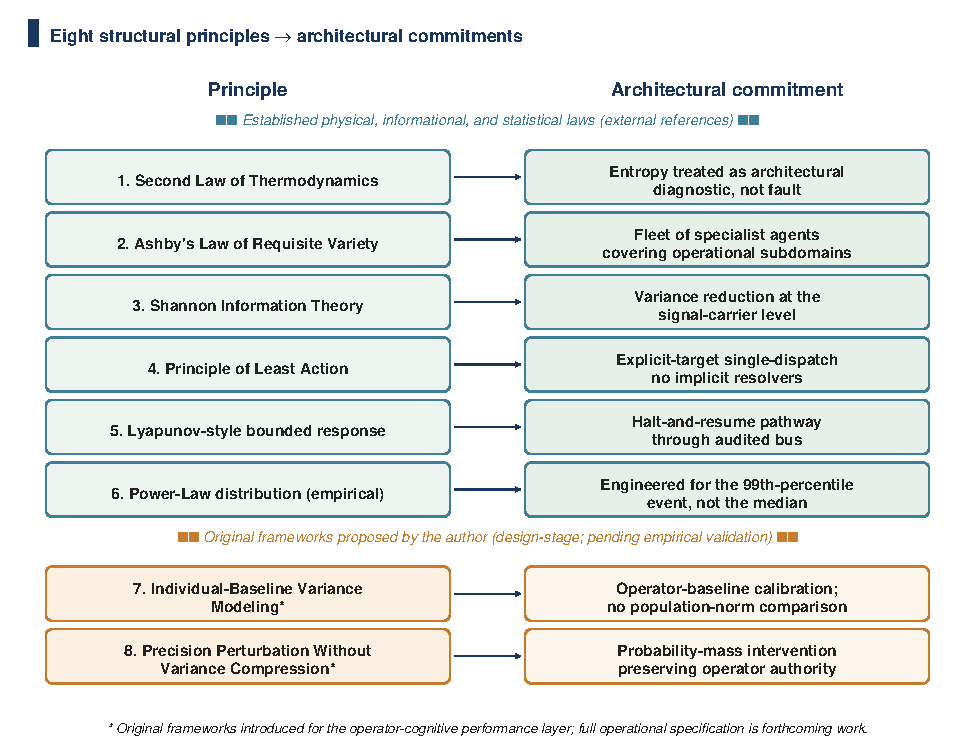
\includegraphics[width=\linewidth]{figures/article4-fig1.pdf}
\end{figure}

\textbf{Selection criterion.} The eight principles are selected against
two filters. \emph{(i)} The principle has a well-developed mathematical
or empirical foundation in its native field --- thermodynamics,
cybernetics, information theory, classical mechanics, control theory,
complex-systems statistics, or (for Principles 7 and 8) cognitive
science. \emph{(ii)} The principle has an operational architectural
form: a design choice in an adaptive AI orchestration system whose
specification can be falsified by observing the system's runtime
behavior. Other foundational principles --- conservation laws, symmetry
principles, dissipation theorems --- satisfy filter (i) but, in the
author's assessment, are difficult to operationalize as architectural
design constraints at the orchestration scale. The eight selected are
not claimed to be the complete set of foundational principles applicable
to adaptive AI; they are the set for which the author can articulate
both the foundation and the architectural form. The framework is open to
extension if additional principles meeting both filters are subsequently
identified.

\textbf{Scope and intent of this paper.} The present paper is a
\emph{perspective paper} --- a synthesis and map across foundations, not
a deep treatment of any single principle. Each of the eight principles
merits its own dedicated technical paper that develops the principle's
operational architectural form in greater mathematical and empirical
detail than space permits here. The contribution of the present paper is
the synthesis: the identification of which principles bound the design
space of adaptive AI orchestration and how each maps to an operational
design choice. Readers seeking deeper treatment of any individual
principle should expect that to be the subject of subsequent work.

\textbf{Orthogonality and overlap among the principles.} The eight
principles are not strictly orthogonal in the mathematical sense; some
derive from or are formally related to others. Most notably, Ashby's Law
of Requisite Variety (Principle 2) can be derived from Shannon's Theorem
10 \cite{ref7}, making Principles 2 and 3 formally related rather than
independent. Lyapunov-style bounded response (Principle 5) and the
thermodynamic-entropy diagnostic (Principle 1) share the structural
concern of bounded behavior under perturbation, viewed from different
physical primitives. The principles are presented as eight because each
has a distinct operational architectural form even where the underlying
foundations are interrelated; the architecture of an adaptive AI
orchestrator that satisfies all eight is structurally over-determined in
a deliberate way, with overlapping constraints reinforcing one another
rather than redundantly stating the same requirement.

\subsubsection{3.1 Principle 1 --- Second Law of Thermodynamics: Entropy
as Architectural
Diagnostic}\label{principle-1-second-law-of-thermodynamics-entropy-as-architectural-diagnostic}

The Second Law establishes that closed systems trend toward maximum
entropy. Applied as an architectural constraint, the principle requires
that entropy be treated as a \emph{diagnostic signal} about system
state, not as a fault condition to be suppressed. Architecturally, this
implies modular construction in which each component can be observed for
entropy drift independently, and in which any component can be replaced
without systemic collapse. In MILO, security drift is detected by an
integrity-monitoring subsystem, carried by the audit-first signal
substrate, and addressed by a bounded incident-response pathway ---
entropy is observed and responded to as information about state. The
architectural consequence is that no subsystem may be a single point of
failure; the failure mode prevented is the monolithic redeploy required
to repair a single drifted component.

\subsubsection{3.2 Principle 2 --- Ashby's Law of Requisite
Variety}\label{principle-2-ashbys-law-of-requisite-variety}

Ashby's law states that a regulator must possess variety at least equal
to the variety of the system it regulates \cite{ref6}. Applied as an
architectural constraint, the principle requires that an AI orchestrator
enumerate response options spanning the operational variety it is meant
to govern. Implementation by a single generalist agent is structurally
insufficient when the operational domain admits distinguishable
subdomains; the orchestrator must instead operationalize a fleet of
specialist agents whose combined variety matches the domain. In MILO, a
fleet of specialist agents --- each registered with a single explicit
role covering an operational subdomain --- provides the requisite
variety against the domains the orchestrator governs; adding variety is
structurally simple, since adding an agent is one new fleet entry while
routing changes remain localized. The failure mode prevented is the AI
orchestrator with five canned responses attempting to govern a domain of
fifty distinguishable states.

\subsubsection{3.3 Principle 3 --- Shannon Information Theory: Variance
Reduction at the Architectural
Level}\label{principle-3-shannon-information-theory-variance-reduction-at-the-architectural-level}

Shannon's information theory bounds the noise-tolerant capacity of any
communication channel \cite{ref7}. Applied as an architectural constraint,
the principle requires that variance reduction occur at the carrier
level --- the signal infrastructure itself --- rather than being
redundantly implemented at each consumer. Architecturally, this implies
a persistent, fanout-aware signal bus that admits reflex-level
interception before subscriber delivery. In MILO, the signal substrate
persists each signal, evaluates reflex predicates, then fans out to
subscribers; reflex arcs run before fanout, short-circuiting
high-severity events at the carrier level. The failure mode prevented is
every consumer reinventing its own noise filter and disagreeing about
what is signal.

\subsubsection{3.4 Principle 4 --- Principle of Least Action:
Single-Target
Dispatch}\label{principle-4-principle-of-least-action-single-target-dispatch}

The Principle of Least Action establishes that physical trajectories
minimize the action integral. Applied as an architectural constraint,
the principle requires that the orchestration path between origin (the
human operator's intent) and target (the responsible component) admit
minimum informational cost --- concretely, no hidden routing layer, no
implicit resolver, no opaque dispatcher. In MILO, every command has one
explicit target; the command bus persists the command, looks up the
target, and invokes the single registered handler. The architectural
patterns are \emph{explicit-target dispatch} and
\emph{persist-before-deliver}: one command, one target, audited before
dispatch \cite{ref1}. The failure mode prevented is command routing through
an opaque resolver where failures cannot be traced to a specific
dispatch --- the failure mode the author observed in pre-MILO
orchestration that motivated the rebuild.

\subsubsection{3.5 Principle 5 --- Lyapunov-Style Bounded
Response}\label{principle-5-lyapunov-style-bounded-response}

Lyapunov's foundational work on stability \cite{ref8} provides the formal
mathematical condition for bounded return-to-equilibrium under
perturbation. The architectural application here is the weaker but
operationally important \emph{Lyapunov-style bounded response}: the
principle requires that any adaptive subsystem admit a bounded response
to disturbance --- concretely, an explicit halt-and-resume pathway that
can be invoked when the subsystem departs its equilibrium zone ---
without claiming a formal Lyapunov-function analysis of the
orchestrator's full state space. In MILO, an emergency-halt reflex
detects critical signals, dispatches a halt command through the command
bus, and symmetrically supports a resume command; every halt and resume
traverses the same audited dispatch path as any other command, with
end-to-end audit entries from critical signal through reflex through
halt-executor. The architectural consequence is that adaptation which
drifts unboundedly is not learning, it is failure; the failure mode
prevented is positive-feedback runaway in an \emph{``adaptive''} loop
that has no architectural stop condition.

\subsubsection{3.6 Principle 6 --- Power-Law Distribution Architecture:
Tail-Event
Preparedness}\label{principle-6-power-law-distribution-architecture-tail-event-preparedness}

Principle 6 differs from Principles 1 through 5 in epistemic status.
Heavy-tailed distributions are an \emph{empirical regularity} observed
across many complex-system domains rather than a derived physical or
mathematical law in the strict sense. Inclusion here is justified under
filter (ii) of the selection criterion above: heavy-tailed consequence
profiles in adaptive AI orchestration are an architectural design
constraint with operational form (engineered for the 99th-percentile
event), regardless of whether the underlying empirical regularity rises
to the status of a law in the philosophical sense.

Empirical statistics in complex systems show that heavy-tailed
distributions dominate consequence profiles \cite{ref9}. Applied as an
architectural constraint, the principle requires that an adaptive AI
orchestrator be engineered for the 99th-percentile event, not the
median. Architecturally, this implies rolling-window degradation
detection (rather than threshold-only alarms), periodic self-monitoring
on a bounded cadence (rather than operator-triggered checks), and
bounded reporting (top-N source ranking) to prevent flooding under tail
events. In MILO, an integrity-monitoring subsystem implements all three:
a health monitor with rolling-window error-and-critical detection per
source, a periodic self-monitoring scheduler on a bounded cadence, and a
signal aggregator that ranks sources by cumulative count without
flooding the dashboard. The architectural consequence is design for the
tail, not the median; the failure mode prevented is the system that
meets 50th-percentile SLO and catastrophically fails at the 99th.

This principle invokes the related concept of \emph{antifragility}
\cite{ref10}: bounded variation and disorder that can improve a system
rather than merely degrading it. The present framing treats
antifragility as an architectural property of the orchestrator's
adaptive-learning loop, not as a generalized claim about humans inside
the system; the application of antifragility-style framings to operators
is addressed in Section 3.8 and Section 4 with explicit governance
constraints.

\subsubsection{3.7 Principle 7 --- Individual-Baseline Variance Modeling
(Original
Framework)}\label{principle-7-individual-baseline-variance-modeling-original-framework}

\textbf{Status --- original framework proposed by the author.} Sections
3.7 and 3.8 introduce frameworks proposed by the author for the
operator-cognitive performance layer of high-consequence adaptive AI
orchestration systems. These frameworks have been submitted to the U.S.
Department of Energy under the Genesis Mission \cite{ref2} and are under
active development. The discussion below is at the principle level.

Established human-factors research has long documented that human error
and operator performance vary across shifts, roles, environmental
conditions, training histories, and task contexts \cite{ref13}, \cite{ref14}.
The original framework proposed here is the architectural application:
an adaptive AI orchestration system that intervenes on the
operator-cognitive performance layer must model variance against the
individual operator's own established performance baseline, not against
a population norm. The architectural form of the principle is:
\emph{Interventions are calibrated to the individual's measured
deviation from their own optimal performance state, established over a
defined baseline window and recalibrated on a defined cadence.} The
failure mode prevented is the AI system that misfires on operators whose
individual baseline differs legitimately from a population norm.

The framework operates under the operational integrity constraints of
\emph{individual consent}, \emph{individual-baseline-only measurement},
\emph{no surveillance architecture}, and \emph{operator authority as the
architectural invariant} \cite{ref1}. Implementation in operational systems
requires institutional ethics review, published consent frameworks, and
periodic third-party audits of system influence patterns and operational
outcomes.

\subsubsection{3.8 Principle 8 --- Precision Perturbation Without
Variance Compression (Original
Framework)}\label{principle-8-precision-perturbation-without-variance-compression-original-framework}

\textbf{Status --- original framework proposed by the author.}
Established cognitive-science and human-reliability work supports
probabilistic modeling of human state, workload, and decision
reliability \cite{ref3}, \cite{ref12}. The original framework proposed here is
the architectural intervention category: \emph{precision perturbation}
--- a class of intervention that shifts probability mass in the
operator's cognitive state distribution toward high-reliability decision
outputs without overriding operator authority and without compressing
the essential variability required for adaptive operational judgment.

The framework is the explicit architectural inverse of two failure modes
commonly observed in operator-facing AI systems: (a) override-style
interventions that bypass operator authority and (b) compression-style
interventions that drive operators toward homogeneous decision states,
eliminating the variability that \emph{is} the operator's adaptive
intelligence. The architectural form of the principle is:
\emph{Interventions are calibrated as precision perturbations to the
operator's probabilistic cognitive state --- neither override nor
compression --- preserving both authority and variability.}

This framework, like Principle 7, operates under the operational
integrity constraints summarized in Section 4 and is currently a v.5
design-stage framework, not yet implemented in shipped MILO code.

\textbf{Operational specification is forthcoming work.} Principles 7 and
8 are introduced here as architectural commitments; their operational
specification --- including the baseline-establishment window for
Principle 7, the recalibration cadence under operator life-events
(illness, role change, circadian variation), the dose-response of the
precision perturbation in Principle 8, and the drift-control mechanism
for the perturbation magnitude over time --- is the subject of
forthcoming work tied to the v.5 development program. The principles
articulate the design target; the operational validation against
measurable outcomes is empirical work that follows from the principles,
not work that precedes them.

\subsection{4. Operational Integrity as Architectural, Not
Policy-Level}\label{operational-integrity-as-architectural-not-policy-level}

The eight principles describe the design space of viable adaptive AI
orchestration. The operator-layer principles in Sections 3.7 and 3.8
admit deployment patterns that, without operational integrity
constraints, would risk surveillance, coercion, or productivity
enforcement. The architecture proposed here requires that those
constraints be \emph{structural}, not merely policy-level ---
implemented as enforceable code-level constraints in deployment builds
and bound to the architectural design specification. The eight integrity
constraints --- \emph{no coercion ever}, \emph{individual baseline
only}, \emph{no surveillance architecture}, \emph{operator authority is
the invariant}, \emph{operational transparency}, \emph{data
sovereignty}, \emph{override always available}, and \emph{independent
oversight} --- must operate as enforceable safeguards, not promises.
Deployment patterns that cannot satisfy all eight are outside the
permitted use boundary of the architecture by design.

\subsection{5. Implications and
Discussion}\label{implications-and-discussion}

Taken together, the eight principles constrain the design space of
viable adaptive AI orchestration more tightly than the field currently
acknowledges. The first six establish that adaptive AI is bounded by
physical, informational, control-theoretic, and statistical constraints
that have been known for between sixty and one hundred and seventy
years. The seventh and eighth extend the framework to the
operator-cognitive performance layer in high-consequence industrial
environments, where human decision context can become a material source
of system variance --- and where the architectural form of the
intervention is precision-targeted rather than population-averaged,
perturbation-based rather than override-based.

The framework is consistent with, and complementary to, several prior
contributions. Friston's Free Energy Principle \cite{ref3} provides a
unified explanation of self-organizing systems at a level above
architectural design; the eight principles operate one level below, as
architectural constraints. Beer's Viable System Model \cite{ref4} applies
cybernetic feedback to recursive viable systems, especially
organizations; the eight principles apply comparable viability
discipline at the software-orchestration scale. Thermodynamics-inspired
AI work \cite{ref5} shows how thermodynamic concepts can illuminate
black-box AI behavior; the present framework treats entropy as
architectural diagnostic. Antifragility \cite{ref10} provides the
payoff-distribution analysis; the present framework treats antifragility
as an architectural property of the adaptive-learning loop bounded by
operator-authority constraints. The synthesis here is intended to
complement, not displace, those frameworks.

The framework leaves substantive work to subsequent contributions on
adjacent architectural concerns: the application of the entropy
diagnostic to multi-source thermal capture for cryptographic seeding,
the application of pre-execution gating to latency-aware authentication
in industrial control environments, the architectural form of
supervisory primacy in human-in-the-loop AI orchestration for
high-consequence domains, and the synthesis of antifragility, viability,
and resilience into a unified design ethos --- each developed in related
work by the author.

\subsection{5.1 Limitations}\label{limitations}

This is a perspective paper synthesizing eight principles. Five specific
limitations bound the present contribution: (i) the mapping of each
established law (Principles 1--6) to a specific orchestrator-level
architectural choice is the author's contribution and is subject to
further validation; alternative mappings are plausible and not surveyed
here; (ii) the relationship of Ashby's Law of Requisite Variety \cite{ref6}
to a fleet of specialist agents is a strong-form analogy rather than a
derived result; (iii) Principle 6 (Power-Law Distribution) is an
empirical regularity rather than a derived law in the strict sense, as
noted explicitly in §3.6; (iv) Principles 7 and 8 ---
\emph{Individual-Baseline Variance Modeling} and \emph{Precision
Perturbation Without Variance Compression} --- are original frameworks
pending empirical validation and are explicitly flagged as design-stage
in §3.7 and §3.8 (their operational specification, including
baseline-establishment windows and dose-response of the perturbation, is
forthcoming work); (v) the synthesis does not claim a unified theory of
intelligence and is explicitly distinguished from Friston's Free Energy
Principle \cite{ref3} in this respect.

\subsection{6. Conclusion}\label{conclusion}

This paper has identified eight structural principles for adaptive AI
architecture. Six are established physical and informational laws
applied as architectural design constraints; two are original frameworks
proposed by the author for the operator-cognitive performance layer. The
principles operate as design-time constraints on architectural choices,
not as a unified theory of intelligence. They constrain the design space
of viable adaptive AI orchestration more tightly than current field
discourse acknowledges. The contribution is at the level of engineering
design --- what an adaptive AI orchestration system must do
architecturally to satisfy the constraints --- and is illustrated using
MILO, the author's working implementation \cite{ref1}, submitted under the
U.S. Department of Energy's Genesis Mission \cite{ref2}. The principles are
intended to be falsifiable, applicable, and consistent with the broader
literature on adaptive systems, cybernetics, and the thermodynamics of
intelligence.

\begin{center}\rule{0.5\linewidth}{0.5pt}\end{center}

\subsection{Data Availability}\label{data-availability}

All architectural materials, source manuscripts, the reference
implementation, and accompanying figures are openly available at
https://github.com/jmontano1/milo-architecture and permanently archived
at Zenodo (DOI:
\href{https://doi.org/10.5281/zenodo.20117025}{10.5281/zenodo.20117025}).
No private datasets are referenced; the architectural framework itself
is the subject of this paper. Patent rights for the underlying MILO
software architecture are reserved; the \textasciitilde MILO trademark
is held under USPTO Serial No.~99706004 (intent-to-use, Class 009).

\subsection{References}\label{references}

\cite{ref1} J. E. Flores Montano, \emph{MILO (Modular Intelligent Learning
Orchestrator)}, JM Automated Solutions. Patent pending. Submitted under
the U.S. Department of Energy Genesis Mission, 2026.

\cite{ref2} U.S. Department of Energy, ``The Genesis Mission: Transforming
Science and Energy with AI,'' Office of the Under Secretary for Science,
Executive Order 14363, November 2025. {[}Online{]}. Available:
https://www.energy.gov/genesis

\cite{ref3} K. Friston, ``The free-energy principle: a unified brain
theory?'' \emph{Nature Reviews Neuroscience}, vol.~11, no. 2,
pp.~127--138, 2010. doi:10.1038/nrn2787

\cite{ref4} S. Beer, \emph{Brain of the Firm}, 2nd ed.~Chichester, UK:
Wiley, 1981.

\cite{ref5} S. Mehdi and P. Tiwary, ``Thermodynamics-inspired explanations
of artificial intelligence,'' \emph{Nature Communications}, vol.~15,
art. 7859, 2024. doi:10.1038/s41467-024-51970-x

\cite{ref6} W. R. Ashby, \emph{An Introduction to Cybernetics}. London, UK:
Chapman \& Hall, 1956.

\cite{ref7} C. E. Shannon, ``A Mathematical Theory of Communication,''
\emph{Bell System Technical Journal}, vol.~27, no. 3, pp.~379--423, July
1948.

\cite{ref8} A. M. Lyapunov, \emph{The General Problem of the Stability of
Motion} (English translation, 1992 reprint of 1892 thesis). London, UK:
Taylor \& Francis, 1992.

\cite{ref9} A. Clauset, C. R. Shalizi, and M. E. J. Newman, ``Power-law
distributions in empirical data,'' \emph{SIAM Review}, vol.~51, no. 4,
pp.~661--703, 2009. doi:10.1137/070710111

\cite{ref10} N. N. Taleb, \emph{Antifragile: Things That Gain from
Disorder}. New York, NY: Random House, 2012.

\cite{ref11} R. Parasuraman, T. B. Sheridan, and C. D. Wickens, ``A model
for types and levels of human interaction with automation,'' \emph{IEEE
Transactions on Systems, Man, and Cybernetics --- Part A: Systems and
Humans}, vol.~30, no. 3, pp.~286--297, May 2000. doi:10.1109/3468.844354

\cite{ref12} E. Hollnagel, \emph{Cognitive Reliability and Error Analysis
Method (CREAM)}. Oxford, UK: Elsevier, 1998.

\cite{ref13} J. Reason, \emph{Human Error}. Cambridge, UK: Cambridge
University Press, 1990.

\cite{ref14} International Atomic Energy Agency, \emph{INSAG-7: The
Chernobyl Accident --- Updating of INSAG-1}, Safety Series
No.~75-INSAG-7. Vienna, Austria: IAEA, 1992.

\begin{center}\rule{0.5\linewidth}{0.5pt}\end{center}

\subsection{About the author}\label{about-the-author}

Jorge Enrique Flores Montano (ORCID iD:
\href{https://orcid.org/0009-0003-1859-8418}{0009-0003-1859-8418};
jmontano@jmautomated.com) is the founder of JM Automated Solutions and
the inventor of MILO. A full biography is maintained at
\url{https://www.milo-usa.com/jorge-enrique-flores-montano.html}.

\subsection{Conflict of Interest and Funding
Disclosure}\label{conflict-of-interest-and-funding-disclosure}

The author is the inventor of MILO (patent pending) and the founder of
JM Automated Solutions. The eight structural principles articulated in
this paper, including the two original frameworks proposed in Sections
3.7 and 3.8, are a contribution from a working development program in
which the author retains sole authorship and inventive interest. No
external funding was received for the preparation of this manuscript.
The author retains all rights to MILO and to the original frameworks
introduced herein.
